\subsection{Designing Change} % (fold)
\label{sub:designing_simple_change}

Table \ref{tbl:storing-data-prog} contains a description of the next program we are going to design. This program will calculate and output the ideal change for a given transaction from a Vending Machine. In designing this program we will make use of the concepts introduced in this chapter; we will use a Function to calculate the coins to give, Variables to store values such as the amount paid, Constants for the values of the different coins, and Parameters to pass values to the Function.

\begin{table}[h]
\centering
\begin{tabular}{l|p{10cm}}
  \hline
  \multicolumn{2}{c}{\textbf{Program Description}} \\
  \hline
  \textbf{Name} & \emph{Change Calculator} \\
  \\
  \textbf{Description} & Calculates the idea change for a given transaction in a Vending Machine. The transaction involves reading the cost of the item purchased and the amount paid, and then outputting the number of each type of coin to give as change.\\
  \hline
\end{tabular}
\caption{Description of the Change Calculator program.}
\label{tbl:storing-data-prog}
\end{table}


To design and implement this program we need to follow a number of steps:
\begin{enumerate}
  \item Understand the problem, and get some ideas on the tasks that need to be performed.
  \item Choose the artefacts we will create and use
  \item Map these artefacts to code
  \item Compile and run the program
\end{enumerate}

In step 1 you need to understand what it is that you want the program to do. This will involve determining the tasks to be performed, the steps involved in those tasks, and any data associated with them. Once you have a good understanding of what you want to achieve you can start to build a solution. In this step you determine the artefacts you want to create, and try to locate those you could use from the available libraries. Step 3 then turns your plans into source code that can be compiled and run in Step 4. 

\begin{figure}[h]
   \centering
   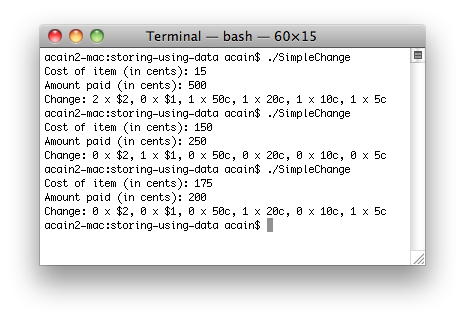
\includegraphics[width=0.4\textwidth]{./topics/storing-using-data/images/SimpleChange} 
   \caption{The Change Calculator running in the Terminal, from \fref{fig:storing-using-simeple-change}}
   \label{fig:storing-using-simeple-change-1}
\end{figure}


% subsection designing_simple_change (end)

\clearpage
\subsection{Understanding the Change Calculator} % (fold)
\label{sub:understanding_simple_change}

Receiving change from a transaction is something that you should be familiar with, and determining the ideal change is not an overly complex task. While the task itself is common, it does not mean that you can skip thinking about it. If you had to give \$6.50 in change you know without thinking that you should give three \$2 coins, and one 50c coin. What you need to do now is think through the steps that you perform intuitively.

Think about all the steps for how you actually calculated the change to be given. The first \emph{secret} is to realise that you need to start with the coin with the largest value, and then work down from there to the coin with the smallest value. The number of coins you give each time can then be calculated by dividing the amount of change to be given by the value of the current coin. Lastly you need to reduce the amount of change that remains to be given. These steps are shown in the pseudocode in Listing \ref{lst:data-simple-change-pseudo}.

\pseudocode{lst:data-simple-change-pseudo}{Pseudocode for Change Calculator program.}{./topics/storing-using-data/application/CalculateChange.txt}
% subsection understanding_simple_change (end)

\clearpage
\subsection{Choosing Artefacts for the Change Calculator} % (fold)
\label{sub:choosing_artefacts_for_simple_change}

The design for any program should involve thinking about the data as well as the tasks involved. You can start by dividing the program's tasks into functions and procedure, and then look at the data that will be needed by these in order to achieve their tasks.

\subsubsection{Designing the tasks for the Change Calculator} % (fold)
\label{ssub:designing_the_tasks_for_the_change_calculator}

Think about the process of calculating change. At the start you need to determine the amount of change that needs to be given. Next you need to determine how many of each kind of coin you are going to give. These steps can be coded into their own functions and procedures. These functions and procedures are outlined in the following list, and shown in the structure chart in \fref{fig:simple-change-structure}.

\begin{itemize}
  \item \texttt{Get Change Value}: This \nameref{sub:function} will be responsible for asking the user to enter the cost of the item, and the amount paid. It will then calculate the amount of change that needs to be given, in cents.
  \item \texttt{Give Change}: This \nameref{sub:procedure} will be responsible for the calculations related to giving one kind of coin as change. This will involve getting the number of coins to give, updating the amount of change remaining, and outputting the details (for that coin) to the Terminal.
  \item \texttt{Coins to Give}: This \nameref{sub:function} will be responsible for calculating the number of coins to give as change, given an amount of change and the value of the coin.
\end{itemize}

\begin{figure}[htbp]
   \centering
   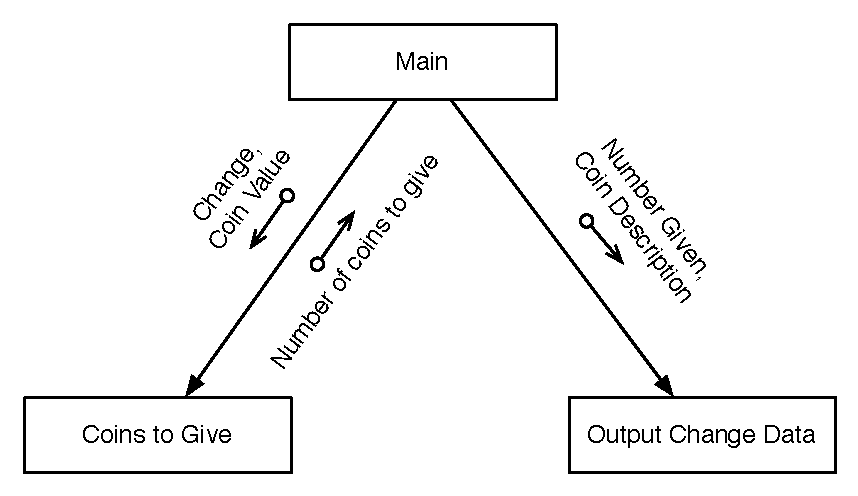
\includegraphics[width=0.6\textwidth]{./topics/storing-using-data/images/SimpleCalcStructure} 
   \caption{Structure Chart for the Change Calculator}
   \label{fig:simple-change-structure}
\end{figure}

To understand how this is going to work you now need to think about how the kinds if data these different tasks are going to need. 

% subsubsection designing_the_tasks_for_the_change_calculator (end)

\subsubsection{Designing the data for the Change Calculator} % (fold)
\label{ssub:designing_the_data_for_the_change_calculator}

Designing data is much like designing the procedures in your program. You need to think about the solution and try to identify the different values that are being used. Each of these values can then become either a Variable, a Parameter, or a Constant. Looking over the steps for calculating change you should be able to identify several different values you will need to work with. You need to be able to store things like the cost of the item being purchased, the amount of money paid, and the amount of change you need to give. A good way to approach this is to think about the values the program will output, as well as the values the user will need to input and any intermediate values you will need to perform the required calculations.

You can use the input/output/processing ideas to help you think about the data that will be required for each function or procedure. Let us examine each of the functions and procedures in turn.

\paragraph{Get Change Value} % (fold)
\label{par:get_change_value}
The first task we can examine if the \texttt{Get Change Value} \nameref{sub:function}. This task will be responsible for determining how much change needs to be given to the user. To design the data needed for this task you can think about its inputs, outputs, and temporary values.

When you are designing a function or procedure it can be given input by the calling code in the \nameref{sub:function_call} or \nameref{sub:procedure call}. Inputs provided via the function or procedure call are coded using \nameref{sub:parameter}s. To determine the parameters you need, think about the information that this function or procedure will need to be given to fulfil its responsibilities. In the case of the \texttt{Get Change Value}, it does not require any input from the caller.

\begin{itemize}
  \item \texttt{Get Change Value} does not require any input from the calling code, so there is no need for any parameters with this function.
\end{itemize}

The \texttt{Get Change Value} task will be coded as a function because it has some output. The result returned by a function is an output, it is what makes it different from a procedure. When you call a function it runs some steps and then returns a value, the value returned is the output from the function. \texttt{Get Change Value} needs to return back the amount of change, this is why it is a function in this design.

\begin{itemize}
  \item \texttt{Get Change Value} returns a number. The number returned is the value of the change to be given in cents.
\end{itemize}

Within the \texttt{Get Change Value} function there will need to be some values that it uses to calculate its output. \texttt{Get Change Value} will need to read the cost of the item from the user, and the amount paid. These two values need to be stored somewhere, so the design of this function will require two \nameref{sub:local_variable}s: they can be called \texttt{Cost of Item} and \texttt{Payment}. These will exist entirely within the function, being the values the function requires to calculate its output.

\begin{itemize}
  \item \texttt{Get Change Value} will have two local variables: \texttt{Cost of Item} and \texttt{Payment}.
\end{itemize}

The pseudocode for this function is shown in \lref{lst:get_change_value}.

\pseudocode{lst:get_change_value}{Pseudocode for the \texttt{Get Change Value} function}{./topics/storing-using-data/application/GetChangeValue.txt}

% paragraph get_change_value (end)

\paragraph{Give Change} % (fold)
\label{par:give_change}
The next task to consider is the \texttt{Give Change} \nameref{sub:procedure}. This procedure will be responsible for coordinating the actions for giving a certain coin in change. Once again you need to think about the inputs it requires (parameters), its outputs, and any values it will work with internally.

Put yourself in the place of the computer.\footnote{Remember the computer is unintelligent. You cannot rely upon your knowledge. Try to think about the information you are using and the steps you are performing to make sure you can capture what needs to be done in your code.} You (as the computer) have been \emph{asked} to \texttt{Give Change}. What data will you need to complete this request? At a minimum you will need to know the total change value that is being given, and the value of the coin that you are issuing.\footnote{In this design the \texttt{Give Change} procedure will be called once for each coin.}

There is one more input that you can only find by thinking about the tasks the computer needs to perform in this code. A part of giving the change will be to output a message, something like `3 x 20c' or `1 x \$2'. The number of coins can be calculated within the procedure, but the text is another issue. The computer will not know what text to output. This data must, therefore, come as input into the procedure.

\begin{itemize}
  \item \texttt{Give Change} needs to be \emph{given} the \texttt{Change Value} variable, and it needs to be told value of the coin and the coin's description. These will be coded as parameters, with \texttt{Change Value} being passed by reference.
\end{itemize}

\texttt{Give Change} will output text to the Terminal, but it also needs to update the \texttt{Change Value} variable it is given. This can be considered as output from the procedure. As the \texttt{Change Value} variable is passed by reference, you can picture this as receiving the variable from the caller. Any changes this procedure makes on its \texttt{Change Value} parameter will actually be changing the value in the variable passed to the \texttt{Give Change} procedure. In this way the procedure is able to output a value.\footnote{An alternative implementation could have been to code this as a \nameref{sub:function}, with the new change value being returned. It would then be the responsibility of the caller to assign this into their change variable.}

\begin{itemize}
  \item \texttt{Give Change} will output the updated \texttt{Change Value}, as this is passed by reference.
\end{itemize}

Within \texttt{Give Change} you will need to store the number of coins to give in change. This will become a local variable that can be used to calculate the updated \texttt{Change Value} and to output the details to the Terminal.

\begin{itemize}
  \item \texttt{Give Change} will have one local variable: \texttt{to give} used to store the number of this coin to be given in the change.
\end{itemize}


The pseudocode for this procedure is shown in \lref{lst:give_change}.

\pseudocode{lst:give_change}{Pseudocode for the \texttt{Give Change} function}{./topics/storing-using-data/application/GiveChange.txt}

% paragraph give_change (end)

\paragraph{Coins to Give} % (fold)
\label{par:coins_to_give}
The \texttt{Coins to Give} function is used to calculate the number of coins to give. This code could have been written within the \texttt{Give Change} procedure, but it was decided to code this in its own function. 

\texttt{Coins to Give} will need to be told the value of the change, and the value of the coin. Both of these parameters will be passed by value, as it is only the values that are required. Internally \texttt{Coins to Give} will not require any additional data, as it can calculate its output from the two input values.

\begin{itemize}
  \item \texttt{Coins to Give} needs to be \emph{told} the value of the change and the value of the coin, it can then use these values to calculate the number of these coins that need to be given in the change.
  \item \texttt{Coins to Give} will output the number of the indicated coin that needs to be given in the change.
\end{itemize}


The pseudocode for this procedure is shown in \lref{lst:coins_to_give}.

\pseudocode{lst:coins_to_give}{Pseudocode for the \texttt{Coins to Give} function}{./topics/storing-using-data/application/CoinsToGive.txt}

% paragraph coins_to_give (end)

\paragraph{Entry Point (Main)} % (fold)
\label{par:entry_point_main_}
The program's code always performs the same task. It coordinates the actions the program is performing. The pseudocode for this was shown in \lref{lst:data-simple-change-pseudo}. This code will need to store the value of the change. It will get the value to store in this by calling \texttt{Get Change Value}. It will call \texttt{Give Change} for each of the coin values, and pass this variable to the procedure for it to update. These actions are shown in \fref{fig:simple-change-seq}.

\begin{itemize}
  \item The \texttt{Entry Point (Main)} needs a local variable to store the \texttt{Change Value}.
\end{itemize}

Thinking further about the program there are also the constant values of the different coins. These values are almost taken for granted when you think about giving change yourself, but remember the computer is unintelligent so you need to specify \emph{everything} for it. The values of the coins can be coded using a constant for each coin. Using constants is a better option than hard coding these values directly in the program, as the name helps provide a context for the value when it is used.

\mynote{
\begin{itemize}
  \item Notice that the functions and procedures are isolated from each other. They have defined inputs and outputs, but their local variables are hidden within their code.
  \item This means you can focus on the function/procedure you are working on, and do not have to think much about the details of the other functions/procedures in your code.
  \item Parameters allow you to pass data into a function/procedure.
  % \item A function returns a value to the caller.
  \item Passing a parameter by reference allows you to output a value by updating the variable you are passed. This means a procedure can output values by having parameters passed by reference, and functions can also use this mechanism to update values in variables as well.
\end{itemize}
}

\begin{figure}[htbp]
   \centering
   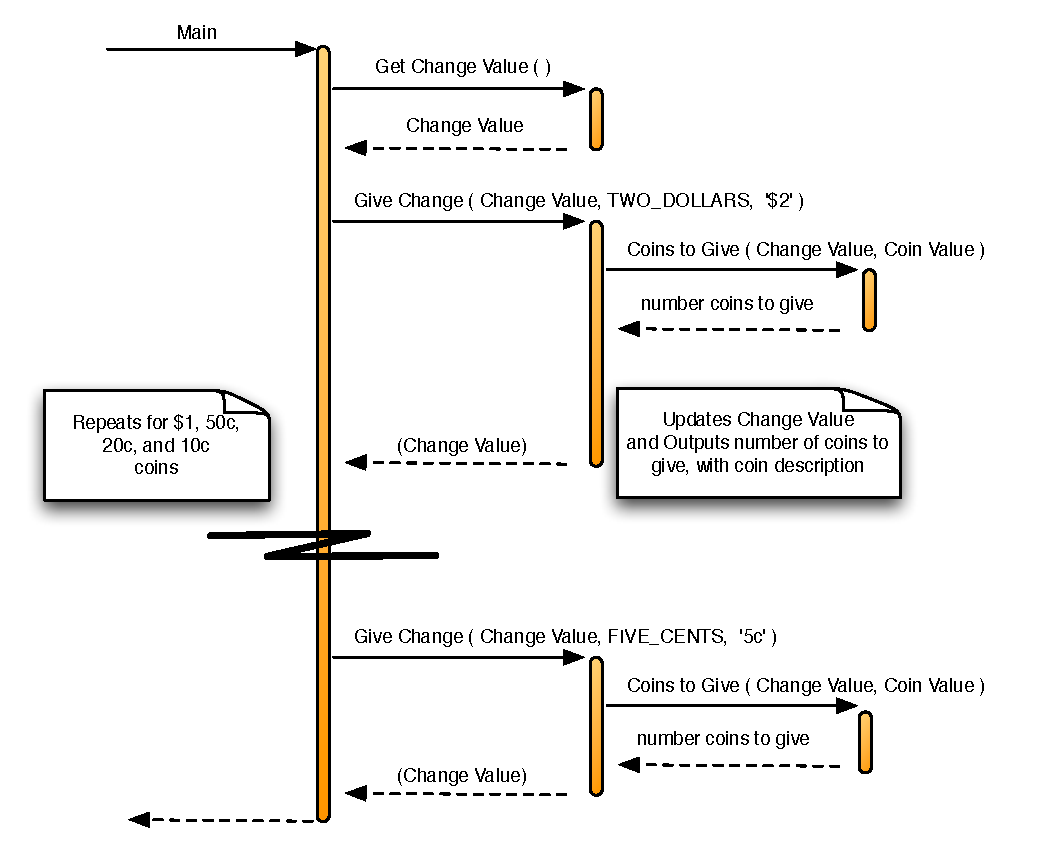
\includegraphics[width=\textwidth]{./topics/storing-using-data/images/SimpleCalcSeq} 
   \caption{Sequence Diagram for the Change Calculator}
   \label{fig:simple-change-seq}
\end{figure}

\clearpage
% paragraph entry_point_main_ (end)
% subsubsection designing_the_data_for_the_change_calculator (end)

\subsubsection{Change Calculator Design Overview} % (fold)
\label{ssub:change_calculator_design_overview}

The Change Calculator program contains the following artefacts:

\begin{itemize}
  \item \textbf{Constants}:
  \begin{itemize}
    \item \texttt{\textbf{TWO\_DOLLARS}} with value 200, represents the value of a \$2 coin
    \item \texttt{\textbf{ONE\_DOLLAR}} with value 100, represents the value of a \$1 coin
    \item \texttt{\textbf{FIFTY\_CENTS}} with value 50, represents the value of a 50c coin
    \item \texttt{\textbf{TWENTY\_CENTS}} with value 20, represents the value of a 20c coin
    \item \texttt{\textbf{TEN\_CENTS}} with value 10, represents the value of a 10c coin
    \item \texttt{\textbf{FIVE\_CENTS}} with value 5, represents the value of a 5c coin
  \end{itemize}
  \item \textbf{Functions}:
  \begin{itemize}
    \item \texttt{\textbf{Get Change Value}}: Calculates and returns the amount of change that needs to be given by the program. This function has the following:
    \begin{itemize}
      \item  \textbf{Local Varaibles}:
      \begin{itemize}
        \item \textbf{\texttt{Cost of Item}}: Stores the value of the item being purchased. This design uses cents as its base to make the calculations easier, avoiding rounding issues involved in using floating point values.
        \item \texttt{\textbf{Payment}}: This is used to store the value of the payment being made. Once again this will be in cents.
      \end{itemize}
    \end{itemize}
    \item \texttt{\textbf{Coins to Give}}: Calculates the number of coins to give, returning how many of these coins should be dispensed as part of giving this change. This has the following:
    \begin{itemize}
      \item  \textbf{Parameters}:
      \begin{itemize}
        \item \texttt{\textbf{Change}}: The value of the change that is to be given.
        \item \texttt{\textbf{Coin Value}}: The value of the coin that is being dispensed.
      \end{itemize}
    \end{itemize}
  \end{itemize}
  \item \textbf{Procedures}:
  \begin{itemize}
    \item \texttt{\textbf{Give Change}}: Calculates the change, and outputs the coin details to the Terminal. This shows the number and description of the change given. This requires the following:
    \begin{itemize}
      \item \textbf{Parameters}:
      \begin{itemize}
        \item \textbf{\texttt{Change Value}} (by reference): The variable that is storing the amount of change to be given.
        \item \textbf{\texttt{Coin Value}}: The value of the coin to issue.
        \item \textbf{\texttt{Coin Description}}: The description of the coin.
      \end{itemize}
      \item \textbf{Local Variables}:
      \begin{itemize}
        \item \texttt{\textbf{To Give}}: Stores the number of the coin to give in change, used to update the \texttt{Change Value} and to output the message.
      \end{itemize}
    \end{itemize}
    \item \textbf{\texttt{Entry Point (Main)}}: this coordinates the overall activity of the program. Getting the amount of change using \texttt{Get Change Value}, and using \texttt{Give Change} to issue the change for each coin.
    \begin{itemize}
      \item \textbf{Variables}:
      \begin{itemize}
        \item \texttt{\textbf{Change Value}}: Keeps track of the current amount of change that has to be given to the user.
      \end{itemize}

    \end{itemize}
  \end{itemize}  
\end{itemize}

In addition to these artefacts the program will make use of some procedures from the available libraries. This will include the following:
\begin{itemize}
  \item \textbf{Output}: You need to use your language's procedures to write output to the Terminal.
  \item \textbf{Input}: Languages also provide a means of reading values from the user. In C and Pascal these input procedures need to be passed the variables that you want the value assigned to. This uses pass by reference to enable the input procedure to store the values read into a variable for you.
\end{itemize}

\csection{
In C the input Procedure to read values from the Terminal is called \csnipet{scanf()}, see \nameref{sub:c_terminal_input}.
}

\passection{
In Pascal the main input Procedure to read values from the Terminal is called \passnipet{ReadLn()}
, see \nameref{sub:pas_terminal_input}.}

% subsubsection change_calculator_design_overview (end)

\subsubsection{Reviewing the design diagrams} % (fold)
\label{ssub:reviewing_the_design_diagrams}

Figure \ref{fig:simple-change-structure} shows the Structure Chart for the Change Calculator. This shows the structure of the solution, visually showing the functions and procedures and the calls between them. This diagram has been enhanced to show the parameter values being passed into the functions and procedures, and the values being returned. These data flows are shown alongside the call arrow, with their own smaller arrow to indicate the direction of the flow. 

By reading Figure \ref{fig:simple-change-structure} you can tell that \texttt{Coins to Give} is going to be a function as it is returning data to \texttt{Main}. \texttt{Give Change} could be a function or a procedure as it is accepting and returning the \texttt{Change Value}, in this design it is a procedure, and updates the value in the \texttt{Change Value} variable using pass by reference. You can also see that \texttt{Coins to Give} and \texttt{Give Change} both require parameters to accept the data being passed into them. 

The Structure Chart shows the static structure of the code, indicating the calls between the functions and procedures, but not communicating when these are called, or how many times. This dynamic information is captured in the Sequence Diagram shown in Figure \ref{fig:simple-change-seq}. This diagram shows the sequence in which the function and procedure calls are performed. Notice that this diagram has also been enhanced to show the data that flows into and out of the functions and procedures. 

The Sequence Diagram indicates how values are being returned. The return of a function's value is shown by indicating the value on the returning arrow. Notice the indication of this value on the arrow returning from the call to \texttt{Get Change Value}, this indicates that \texttt{Get Change Value} is a function. On the other hand, the brackets around the return value from \texttt{Give Change} indicates that this is being performed by updating a parameter that was passed using pass by reference. You can use this information to determine how the design intends these to be coded. As \texttt{Get Change Value} is directly returning a value it must be a function, \texttt{Give Change} updates a parameter and does not return a value itself so it must be a procedure.

\mynote{
\begin{itemize}
  \item A structure chart shows the static structure of the program. This tells you which procedure/functions call which, and the data that is passed between them. It shows you what is written in the code.
  \item A sequence diagram shows the dynamic operation of a program. This tells you how the functions and procedures interact to achieve some goal. It shows you what is happening when the code is run.
\end{itemize}
} 

% subsubsection reviewing_the_design_diagrams (end)

\clearpage
\subsubsection{Designing data in general} % (fold)
\label{ssub:designing_data_in_genera}

When you are designing a program you need to think about each function or procedure, and determine if it requires data to be given to it to enable it to perform its action. Any data it requires must then be passed to it using Parameters. The key to understanding parameters is to remember that each function/procedure is its own isolated domain. It can have its own data, using local variables, and has its own instructions. In most cases these instructions will need to be given some starting data, some information upon which to act. 

One strategy you can use to picture this is to put yourself in the place of the function, or procedure. For example, what would you need to be told in order to determine the number of coins to give in change for a single coin type. You can not work out the answer without being told the value of the change to be given, and the value of the coin. With these two pieces of information you now have enough to calculate the required output. For example, how many \$2 coins should be given for \$6.50 in change. These two pieces of data can be used to calculate the answer 3. This is exactly what is being coded in the \texttt{Coins to Give} function.

In this respect Procedures are the same. In order to give change, the \texttt{Give Change} procedure needs some information. It can not act without this information. If you needed to \emph{give change}, you need to be told something about the amount of change you are giving and the value of the coin you are issuing. In this case, \texttt{Give Change} needs to be told the \texttt{change value}, the \texttt{coin value}, and the description of that coin. With these details the procedure can then code the steps needed to produce its desired side effects.

Parameters are mostly used to pass a value into a function or procedure. However, in some cases it is useful to pass in the \emph{variable} rather than the \emph{value}. This is the case when you want the function or procedure to \emph{change} the value in the variable passed to it. Take the \texttt{change value} parameter in \texttt{Give Change} as an example. When this procedure issues some coins, the amount of change still to be given must be updated. For example, when you issue `3 x \$2' for the \$6.50 in change, the new change value will be 50c ($650 - (3 \times 200)$). By passing the \emph{variable} into \texttt{Give Change} it is possible for this code to change the value in the callers variable, ensuring that the correct change is given.

% subsubsection designing_data_in_genera (end)

\subsubsection{Modelling and Abstraction} % (fold)
\label{ssub:modelling_and_abstraction}

One of the main keys to understanding programs, and to creating good designs, is to see how each artefact you create models something from the problem. The procedures that you create model the processes, performing actions that relate to the task at hand. The functions model calculations that need to be performed, such as determining how many coins should be given. In the same way the variables that you create will store values related to the problem. Each variable \textbf{represents} something, some information related to your program. The \emph{thing} it represents should be reflected in the name given to the variable.

The act of trying to model the problem in software is called \textbf{abstraction}. It is the process of determining the features of the problem that are essential to the solution, and capturing these in a way that models reality but keeps only the details we care about. The ability to create your own model is a skill that you learn with experience, taking a lot of practice to really master.

\mynote{
\begin{itemize}
  \item A good design will closely model the program's domain. You should be able to relate the artefacts you are creating with things related to the program.
\end{itemize}
}

% subsubsection subsubsection_name (end)
% subsection choosing_artefacts_for_simple_change (end)

\clearpage
\subsection{Writing the Code for the Change Calculator} % (fold)
\label{sub:writing_the_code_for_simple_change}

The pseudocode from Listing \ref{lst:data-simple-change-pseudo} shows the instructions, and how these should be divided between the \texttt{Coins to Give} Function and \texttt{Output Change Data} Procedure. At this stage these instructions need to be translated into source code, so that they can be compiled and the resulting program tested.

The following two sections, Section \ref{sec:storing_and_using_data_in_c} \nameref{sec:storing_and_using_data_in_c} and Section \ref{sec:storing_and_using_data_in_pascal} \nameref{sec:storing_and_using_data_in_pascal}, contain a description of the syntax needed to create programs in the C and Pascal programming languages that include Variable and Function declarations.

\mynote{
Remember the basic process for reading the Syntax Diagrams is to:
\begin{enumerate}
  \item Find the page with the Syntax rule you are interested in knowing about.
  \item Have a quick look at the Syntax Diagram and the rules it contains. Read each rule, and get a basic feel for how it is going to come together for your program.
  \item Read the example to see one way of using the Rule. The Syntax Diagram can be used to create any number of variations of the rule, the example gives you at least one way these rules can be coded.
  \item Return to the diagram and make sure you can match each part of the example back to the rule that created it.
  \item Look up any related rules that are not explained on this rule's page.
\end{enumerate}
}
% subsection writing_the_code_for_simple_change (end)

\clearpage
\subsection{Compiling and Running the Change Calculator} % (fold)
\label{sub:compiling_and_running_simple_change}

Once you have completed your program, you need to compile and test it. 

\begin{enumerate}
  \item Open the \textbf{Terminal}\footnote{The \textbf{MinGW Shell} on Windows.} program for your Operating System
  \item Use the \texttt{\textbf{cd}} command to move to the directory with your code, for example \newline \bashsnipet{cd /Users/acain/Documents/Code}
  \item Run the compiler with your program's code. See the language specific details below.
  \item Fix any compiler errors, using the tips from Section \ref{ssub:compiler_errors} \nameref{ssub:compiler_errors}.
  \item Execute the program using \bashsnipet{./SimpleChange} and check the results
\end{enumerate}

\csection{
The C compiler is called \textbf{gcc}. To compile your \emph{Change Calculator} program you will need to run the following: \newline \newline \bashsnipet{gcc -o SimpleChange simple-change.c}
}

\cppsection{
C does not have support for pass by reference, though it can be achieved using other means (see \cref{cha:dynamic_memory_allocation}). The C++ language is an extension to C that fixed a number of issues, as well as added some new features. One of the new features was built in pass by reference. To compile the C++ version of the Change Calculator you need to use the C++ compiler called \textbf{g++}. To compile your \emph{Change Calculator} program you will need to run the following: \newline \newline \bashsnipet{g++ -o SimpleChange simple-change.cpp}
}

\passection{
The Pascal compiler is called \textbf{fpc}. To compile your \emph{Change Calculator} program you will need to run the following: \newline \newline \bashsnipet{fpc -S2 SimpleChange.pas}
}

\clearpage
\subsubsection{Generating Test Data} % (fold)
\label{ssub:generating_test_data}

Now that our program is making greater use of data it becomes more important to think about how to test your program. Testing is the process of trying to locate issues with your code. There are two main classifications for issues, \textbf{syntactic errors} and \textbf{semantic errors}.

Syntactic errors indicate places in your code where you have not correctly followed the syntax of the language. These are the easiest kind of error to find as the compiler will not be able to compile the program if its syntax is not correct. The errors that the compiler report are all syntax errors. As you gain experience with a Language you will find that you make fewer and fewer of these kinds of errors. 

Semantic errors, on the other hand, will not be found by the compiler. These are errors in the logic within the program. They are cases where you have correctly structured the code, but the code itself does not get the computer to perform the actions you require. These are the kinds of errors that you need to learn to be able to detect yourself. Selecting the right kind of test data is an important task when you start to think about testing programs.

For the Change Calculator there are two inputs provided by the user. In order to test this program you need to determine the values that are passed to the \texttt{Cost of the Item} and the \texttt{Payment} inputs. You want to choose values that can help you uncover any unexpected issues with the programs code.

\begin{table}[htbp]
\begin{tabular}{|l|l|l|p{7cm}|}
  \hline
  \textbf{Cost of Item}  & \textbf{Payment} & \textbf{Expected Output}  &   \textbf{Reason} \\
  \hline
  \$2.50 & \$5.00 & 1 x \$2, 1 x 50c & Basic test to check that the program works for a simple data input. \\
  \hline
  \$0.15 & \$4.00 & 1 of each coin & Generates \$3.85 in change, checking that each coin is used. \\
  \hline
  \$0.05 & \$0.10 & 1 x 5c & Check the output can be a single coin. Could also add tests to check other individual coins. \\
  \hline
  \$0.60 & \$1.00 & 2 x 20c & Check that 2 coins can be given. \\
  \hline
  \$0.00 & \$5.00 & 2 x \$2, 1 x \$1 & Can it accept no cost of item, and give back payment? \\
  \hline
  \$3.85 & \$0.00 & -1 of each coin & Check what happens if insufficient funds are provided. \\
  \hline
\end{tabular}
\caption{Test Data for the Change Calculator}
\label{tab:simple_change_test_data}
\end{table}

The data we use to test an execution of a program is called a \textbf{Test Case}. Each test case provides a set of input values, and the expected results given this input. Example test cases for the Change Calculator are shown in Table \ref{tab:simple_change_test_data}. This table shows the input values, the expected output values, and some rational for why this test case should be run. To perform the testing you run the program once for each test case and check the output of the program against the expected output. If there are any differences you know that their is a problem, and need to check the program's code to find the source of the logic errors.




% subsubsection generating_test_data (end)

% subsection compiling_and_running_simple_change (end)